\documentclass[runningheads,a4paper]{llncs}
\usepackage{llncsdoc}
\usepackage{subfigure}
\usepackage{amsmath}
\usepackage{amssymb}
\setcounter{tocdepth}{3}
\usepackage{graphicx}
\usepackage{booktabs}
\usepackage{times}
\usepackage{url}
\urldef{\mailsa}\path|qiutie@ieee.org|
\newcommand{\keywords}[1]{\par\addvspace\baselineskip
\noindent\keywordname\enspace\ignorespaces#1}

\begin{document}

\mainmatter  % start of an individual contribution

% first the title is needed

\title{A New Energy-efficient Time Synchronization Algorithm}

% a short form should be given in case it is too long for the running head
\titlerunning{ }

% the name(s) of the author(s) follow(s) next
%
% NB: Chinese authors should write their first names(s) in front of
% their surnames. This ensures that the names appear correctly in
% the running heads and the author index.
%




\author{Weidong Guo$^1$%
\and Tie Qiu$^{1,2,*}$\and Lei Wang$^1$\and Jie Liu$^1$\and Chengdang Song$^1$}
%
\authorrunning{ }
% (feature abused for this document to repeat the title also on left hand pages)

% the affiliations are given next; don't give your e-mail address
% unless you accept that it will be published
\institute{$^1$School of Software, Dalian University of Technology, Dalian, 116620, China\\
$^2$Electrical and Computer Engineering, Iowa State University, Ames, IA 50010, USA
\mailsa}


\toctitle{Lecture Notes in Computer Science}
\tocauthor{Authors' Instructions}
\maketitle


\begin{abstract}
In recent years, issues of Wireless Sensor Networks (WSNs) have been widely studied. The energy is limited in WSNs. However, it always takes much energy to achieve highly accurate time synchronization. In this paper, a Spanning Tree-based Energy-efficient Time Synchronization (STETS) strategy for WSNs is proposed. In STETS, only a small number of sensor nodes in the WSN have the privilege to send messages and each of these nodes sends only one broadcast in a single round of time synchronization. By taking advantage of the intersection and difference set of these broadcasts' domains, a spanning tree structure will be created in the WSN. By using the information carried by these broadcasts, time synchronization process will also be completed. We simulate and evaluate the performances of the algorithm on NS2. The experiment results show that our algorithm is efficient in both energy consumption and accuracy of time synchronization.
\keywords{ time synchronization, wireless sensor networks, spanning tree}
\end{abstract}

\section{Introduction}
The correct and efficient operation of many applications and protocols \cite{1,2} in WSNs requires a common time scale. In order to fulfill this demand, sensor nodes are required to communicate with each other and establish a logical clock which represents global time. However, WSNs have many weaknesses such as limited energy, limited handling capacity, limited communication capacity, limited storage capacity, etc. These problems bring difficulties to the researches on time synchronization.

Accurate time synchronization algorithms result in accurate coordination and collaboration of sensor nodes. However, many early proposed approaches focus so much on cutting down time synchronization error that they also cause serious energy consumption. In \cite{3}, RBS which is a time synchronization approach based on Receiver to Receiver Protocol (RRP) is proposed. It requires that each node in a cluster must calculate time offset of every other node in the cluster. This would bring large storage and calculation burden to the entire network, and thus a considerable amount of energy would be wasted. Two synchronization approaches based on Sender-to-Receiver Protocol (SRP) were proposed in \cite{4}: Tiny-Sync and Mini-Sync. In order to approximately fix the frequency of each clock, a large number of message exchanges and intensive computation are required. Other approaches such as \cite{5,6,7} also do not take into account the limited energy available for sensor networks either due to redundant network traffic or over-complicated computing. Furthermore, in sensor network applications where the number of sensors is large and the desired area is small, the lifetime of the entire networks will decrease sharply due to frequent message exchanges. Thus, message number should be limited when designing time synchronization approaches in densely connected WSNs.

In this paper, we incorporate the RRP and SRP to present a novel energy-efficient time synchronization approach, namely STETS. Our approach takes advantage of the property of RRP, namely being able to synchronize a large number of nodes at one time. This can help reducing number of messages and thus energy. Also, by using SRP, STETS successfully synchronize the unsynchronized nodes caused by RRP. In STETS, only a small number of nodes in WSNs have the right to send information and each of these nodes only needs to send one message in a single round of time synchronization. Moreover, all the messages in our approach are in the form of broadcast for the purpose of decreasing protocol overhead. Thus, energy-efficiency can be ensured in STETS.


The rest of this paper is organized as follows: In section 2, we present the system model of our algorithm. In section 3, we give our algorithm design. In section 4, we simulate STETS and other two approaches and present comparisons on time synchronization error and energy consumption. Finally, we give our conclusion in section 5.

\section{Model and Strategy}
\subsection{Assumption}
We assume that the sensor nodes have unique identifiers. Each node is aware of the set of nodes with which it can directly communicate. These nodes are also termed as the neighboring nodes. We also assume that each node knows the distance to each of its neighboring nodes. This can be achieved through various distance estimation algorithms such as TOA (Time of Arrival) \cite{8}, TDOA (Time Difference of Arrival) \cite{9}, RSSI (Received Signal Strength Indicator) \cite{10}.

\begin{figure}[h]
\centering
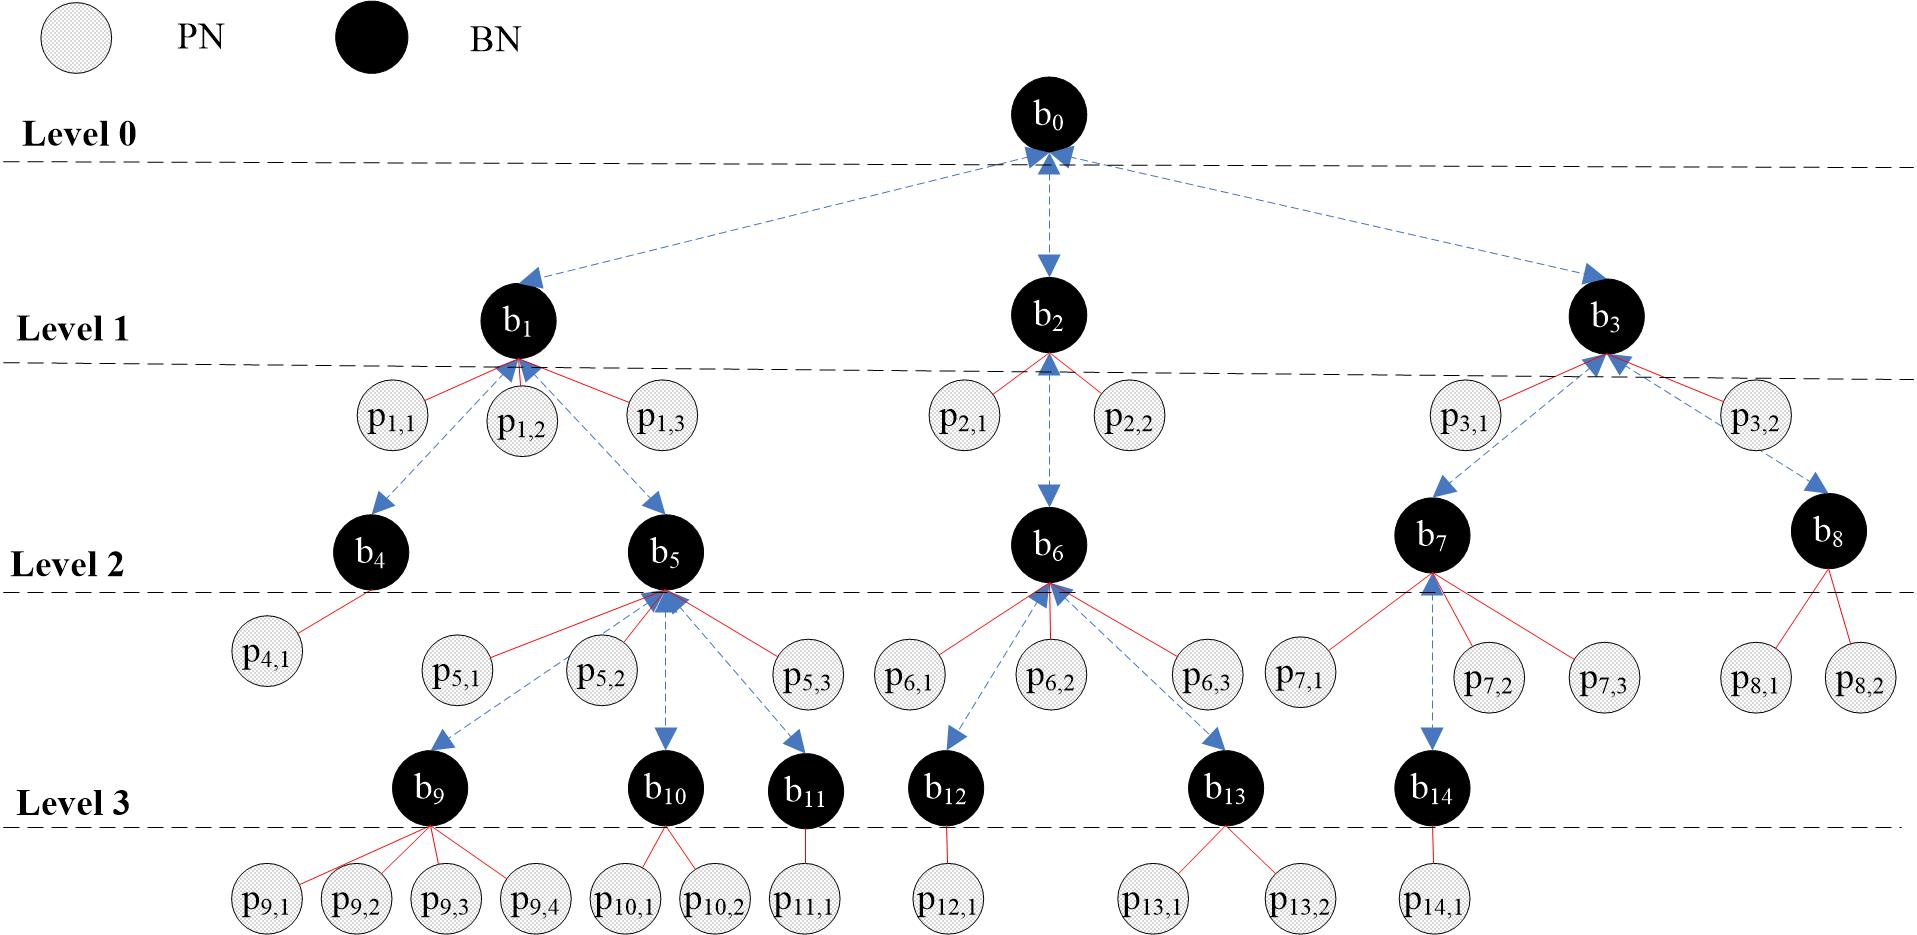
\includegraphics[width=4.0in]{fig1.jpg}
\caption{Spanning tree structure in WSNs}
\label{fig_sim}
\end{figure}

\subsection{Node Classification}
The sensor nodes in the entire WSNs are classified into three categories: undefined node (UN), backbone node (BN) and passive node (PN). Let $ b_{i}$ ($i\geq 0$) denote the BN; let $ p_{i,j}$ ($i\geq 0,j\geq 1$) denote the PN which is the slave node of $ b_{i}$; The explanations of these nodes are as follows:
\begin{itemize}
\item \textbf{Undefined node (UN)}: the initial state of each node in WSNs. These nodes will become either BN or PN during the time synchronization.
\item \textbf{Backbone node (BN)}: the nodes of this state form a spanning tree structure in the network (Figure 1). One certain BN on level $l$ ($0<l\leq n$) can communicate with only one BN on level $l-1$ and the BN on level $l$ synchronizes with the BN on level $l-1$ through SRP. In the spanning tree, every branch node or root node has one or more child nodes. Not all the leave nodes are distributed on the last level.
\item \textbf{Passive node (PN)}: each BN except for the one on level 0 takes charge of a group of nodes which are called PNs (Figure 1). These PNs do not belong to any level. By listening to the communication among BNs, these PNs synchronize with their master node, namely the BN who takes charge of them.
\end{itemize}


If a BN on level $l$ ($0<l\leq n$) synchronizes with a BN on level $l-1$, the former is the child node of the latter while the latter is the father node of the former. If a PN synchronizes with a BN, the former is the slave node of the latter while the latter is the master node of the former. It should be noted that the BN on level 0 has neither father node nor slave node.

\subsection{Message Format}


There is only one type of message called \textit{Sync} in the form of broadcast in STETS for the purpose of reducing complexity. The following are the contents of the message:

\begin{itemize}
\item \textit{ID}: the unique identifier of the sender who broadcasts this \textit{Sync} message.
\item \textit{FatherID}: the unique identifier of the sender's father node.
\item $ L$: the level on which the sender lies.
\item \textit{RT}: If the sender has already received a \textit{Sync} message from its father node and recorded the timestamp at its arrival, the \textit{RT} should not be \textit{NULL} but be filled with the timestamp.
\item \textit{ST}: the timestamp the sender records when sending this \textit{Sync} message.
\end{itemize}


\section{Algorithm Design}
\label{sec:algorithm}

In STETS the layering and time synchronization are carried out together. At the time when all the BNs and PNs have been elected in WSNs, time synchronization of all the nodes has also been completed.

\subsection{BNs and PNs Election}

In our approach, the BNs and PNs election process is divided into three
phases.

Phase 1: at the beginning of the round of time synchronization, the randomly elected $ b_{0}$ broadcasts a \textit{Sync} message to all the UNs in the broadcast range. Each of these UNs setups a timer after it receives the \textit{Sync} message. The initial value of the timer is inversely proportional to the distance between the UN and $b_{0}$. In this way, elected BNs can be relatively evenly distributed in the WSNs.

Phase 2: when the timer of one certain UN expires, the node becomes a BN. It assigns itself a level, one greater than the level it has received. Then the node broadcasts a \textit{Sync} message.


Phase 3: Each UN who has received the \textit{Sync} message in phase 2 checks the FatherID field. If the UN has already received a \textit{Sync} message from the BN having the identifier FatherID, It will immediately cancel its running timer. And the UN becomes a PN of the BN who sent the message in phase 2. The PN will ignore any other \textit{Sync} message during the round of synchronization. Otherwise, the UN will setup a timer.

\begin{figure}[h]
\centering
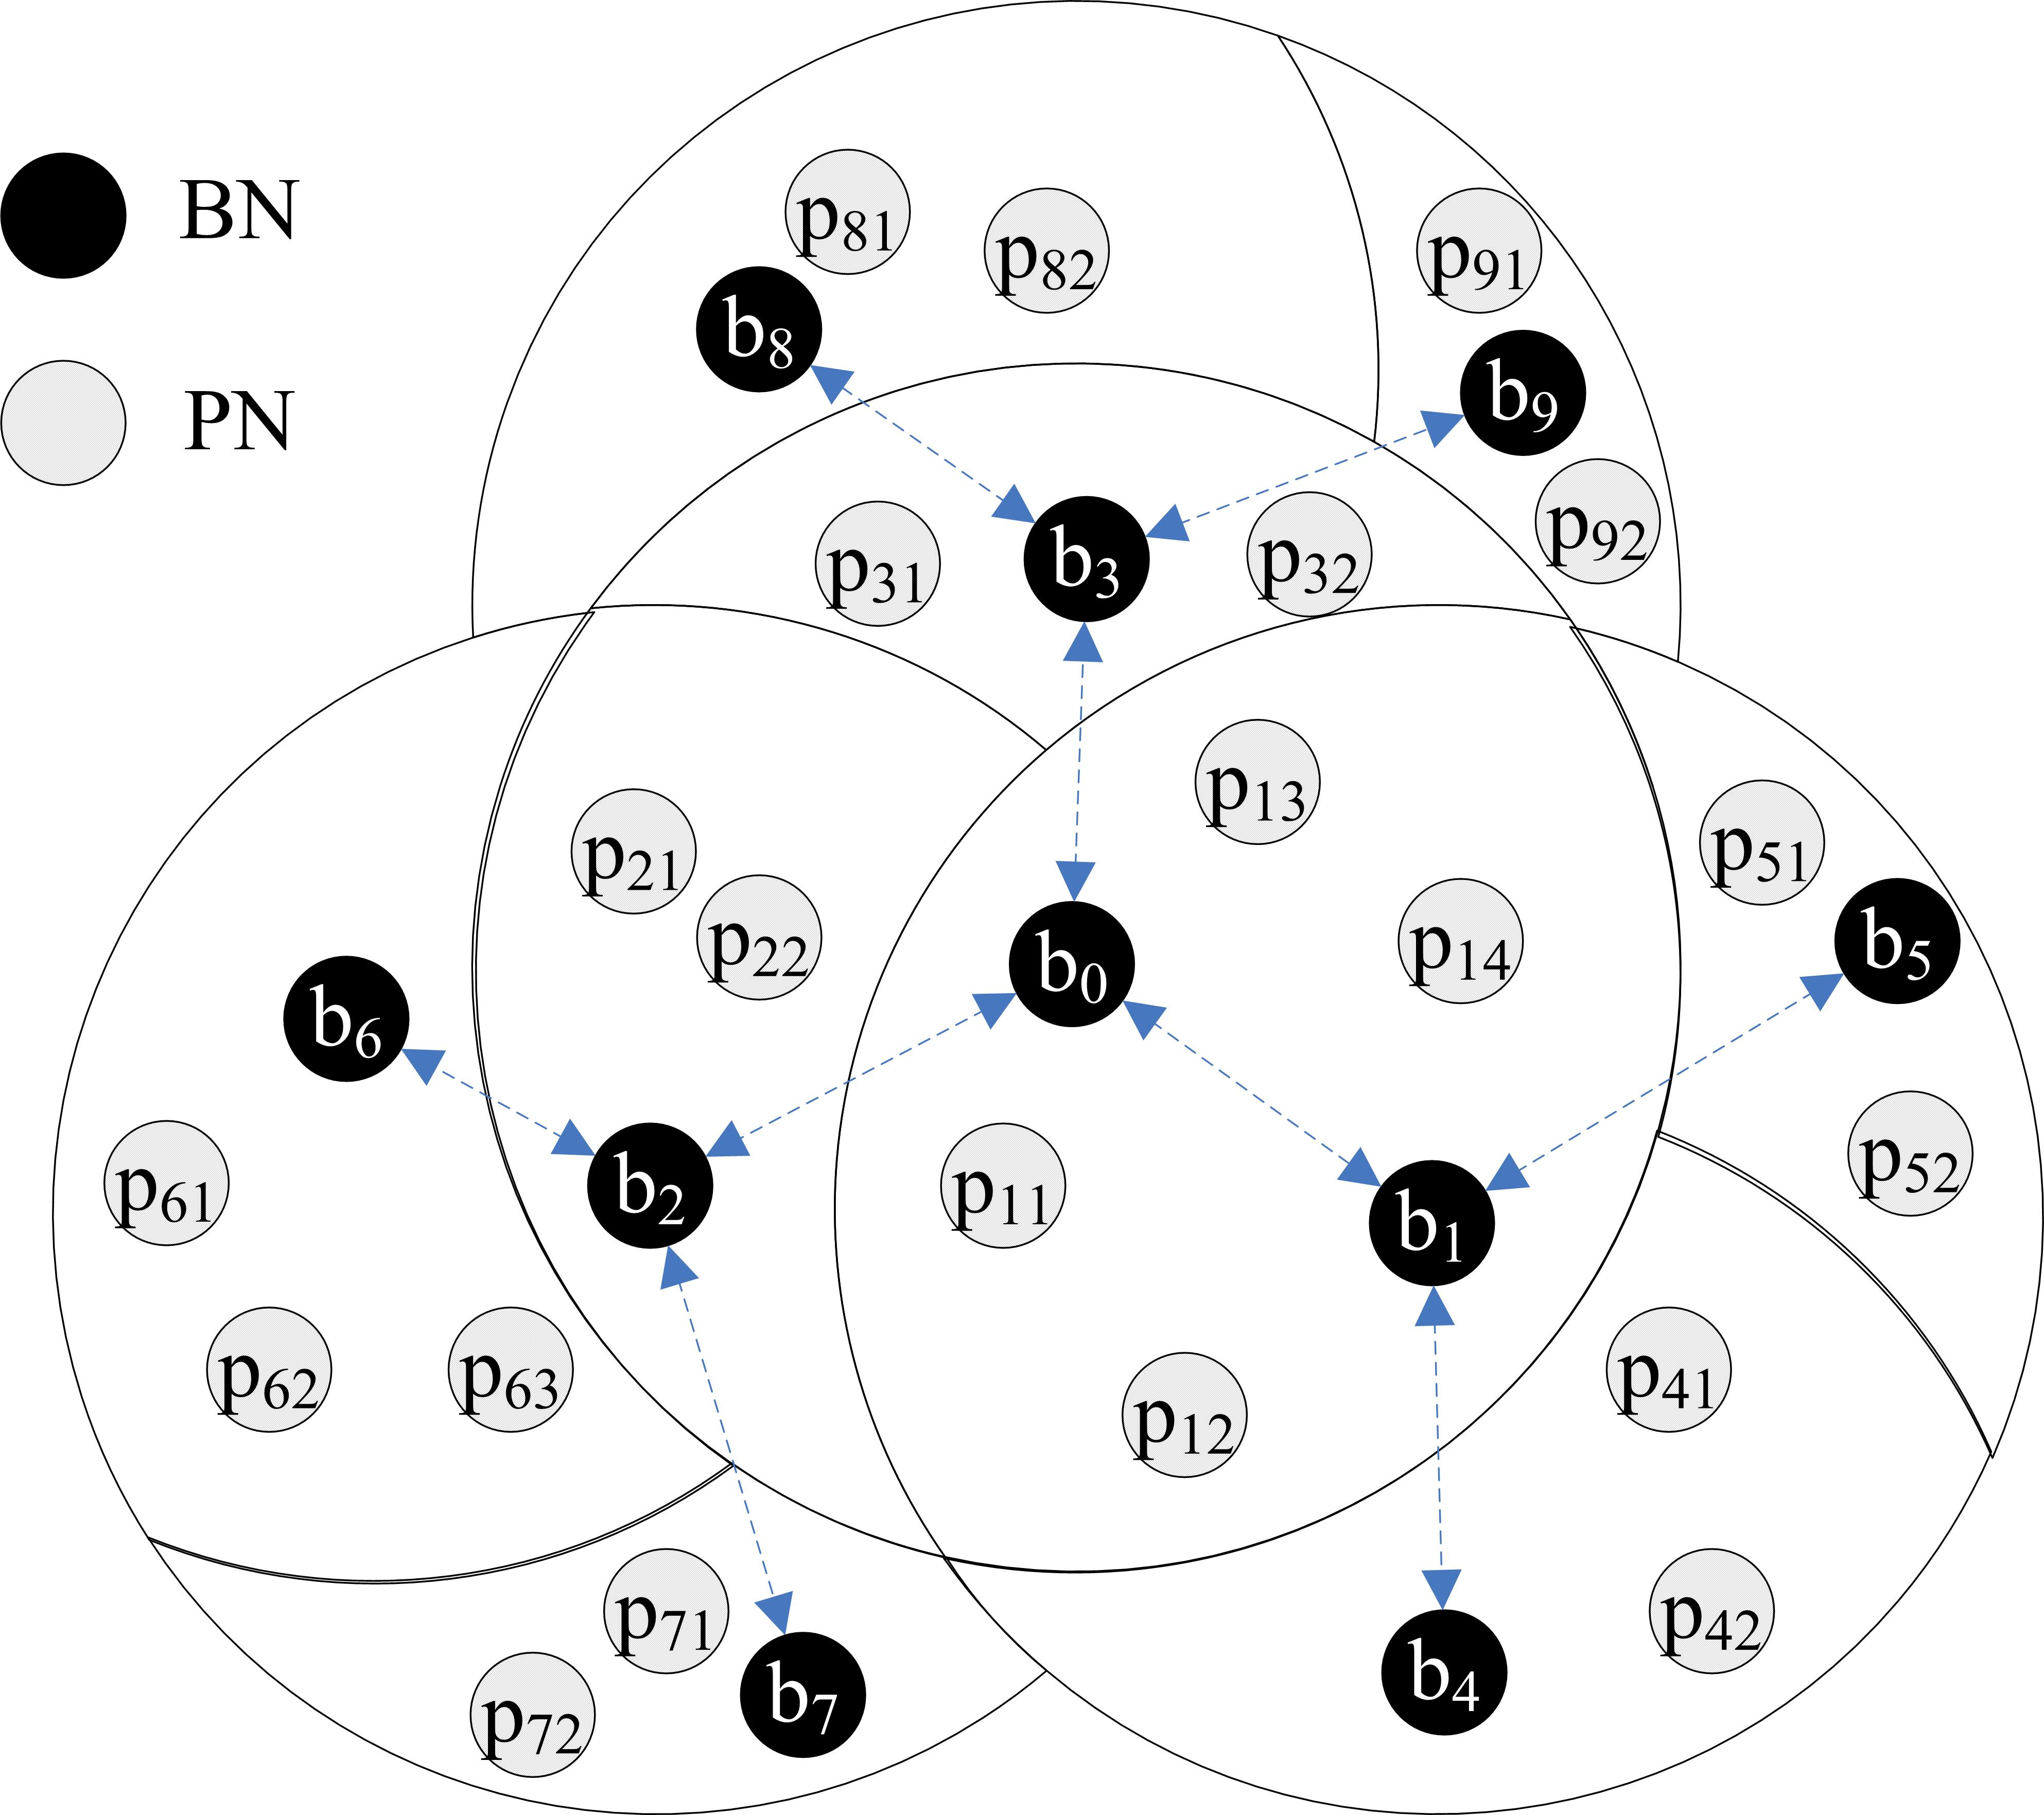
\includegraphics[width=2.5in]{fig2.jpg}
\caption{WSNs topology using STETS}
\label{fig_sim}
\end{figure}

Then the phase 2 and 3 will be executed repeatedly until the last BN broadcasts a \textit{Sync} message and it does not receives any \textit{Sync} message from its child node. This means no child BN will be generated and no \textit{Sync} message will be broadcasted. At that time, each UN in the network has become either a BN or a PN. Finallly, a topology shown in Figure 2 will be created. 31 UNs becomes 9 BNs and 22 PNs. The 9 BNs form a 3-level spanning tree structure in the WSNs.





\subsection{Time Synchronization}
When an UN becomes BN, it will broadcast \textit{Sync} message. By taking advantage of the time and identifier information contained in the \textit{Sync} messages, time synchronization can also be achieved.

Assume there is a BN $ b_{i}$ ($i\geq 0 $) on level $l$ ($l\geq 0 $) and it has a child node $b_{j}$ ($j\geq 0 $) on level $l+1$. There also exist a group of PNs $p_{j,x}$ ($x\geq 1 $) which are slave nodes of $b_{j}$. The \textit{Sync} message broadcasted by either $b_{i}$ or $b_{j}$ can certainly be received by $p_{j,x}$ according to the BNs and PNs election. Let \textit{sync1} and \textit{sync2} respectively represent the \textit{Sync} messages from $b_{i}$ and $b_{j}$.


\begin{enumerate}
\item \textit{BN Time Synchronization}: $ b_{i}$ synchronizes with $ b_{j}$ via the algorithm provided in SRP \cite{5}. At the time when \textit{sync1} is broadcasted, a timestamp $ T_{1}$ is recorded by the local clock of $ b_{i}$. \textit{sync2} contains two timestamps $ T_{2}$ in the \textit{RT} field and $ T_{3}$ in the \textit{ST} field. When \textit{sync2} is received by $ b_{i}$, the BN records a timestamp $ T_{4}$. Then, $ b_{i}$ can calculate the time offset between $ b_{i}$ and $ b_{j}$ through $ T_{1}$, $ T_{2}$, $ T_{3}$, $ T_{4}$:

\begin{equation}
\label{eq1}
\Delta_{b_{i} \to b_{j} } =\frac{\left( {T_{2} -T_{1} }
\right)-\left( {T_{4} -T_{3} } \right)}{2}
\end{equation}

Using the time offset, $ b_{i}$ and $ b_{j}$ can synchronize with each other.

\item \textit{PN Time Synchronization}: $p_{j,x}$ synchronizes with its master node $ b_{j}$ via the algorithm provided in RRP \cite{3}. At the time when \textit{sync1} is broadcasted, a timestamp $ T_{5}$ is recorded by the local clock of $p_{j,x}$. By eavesdropping the \textit{sync2}, $p_{j,x}$ knows the timestamp $ T_{2}$. Thus, $p_{j,x}$ can calculate the time offset between $p_{j,x}$ and $ b_{j}$ through $ T_{2}$, $ T_{5}$:

\begin{equation}
\label{eq4}
\Delta_{p_{j,x} \to b_{j} } =T_{2} -T_{5}
\end{equation}

$p_{j,x}$ uses such time offset to synchronize with $ b_{j}$. In the end, each PN will synchronize with its master node while each BN except for $b_{0}$ will synchronize with its father node.

\end{enumerate}


\section{Simulation and Performance Evaluation}
\subsection{Simulation Setup}
We evaluated the performance of our proposed algorithm by performing STETS and other approaches using the network simulator NS-2. These approaches include Time synchronization based on spanning tree for wireless sensor networks (TSBST) \cite{6} and TPSN \cite{5} which are both based on spanning tree structure for WSNs. The simulation scenario was set as follows: 240 nodes were deployed randomly in a 500mX500m area in which the network density varies as 10, 20, 30, 40, 50 and 60. Here, we define the network density as the average number of neighboring nodes of each sensor node. The density was controlled by setting the communication range.

Our evaluation metrics are energy consumption, global and local time synchronization error. We performed 10000 cycles of time synchronization for each network and we averaged the observed values of these cycles. Each time synchronization cycle lasts 10 seconds because this duration is sufficient for all the nodes in the network to be synchronized and for all the necessary broadcasts to avoid collision. Each message for the three approaches is in the form of broadcast for the purpose of ensuring fairness.

\begin{figure}[!h]
\centering
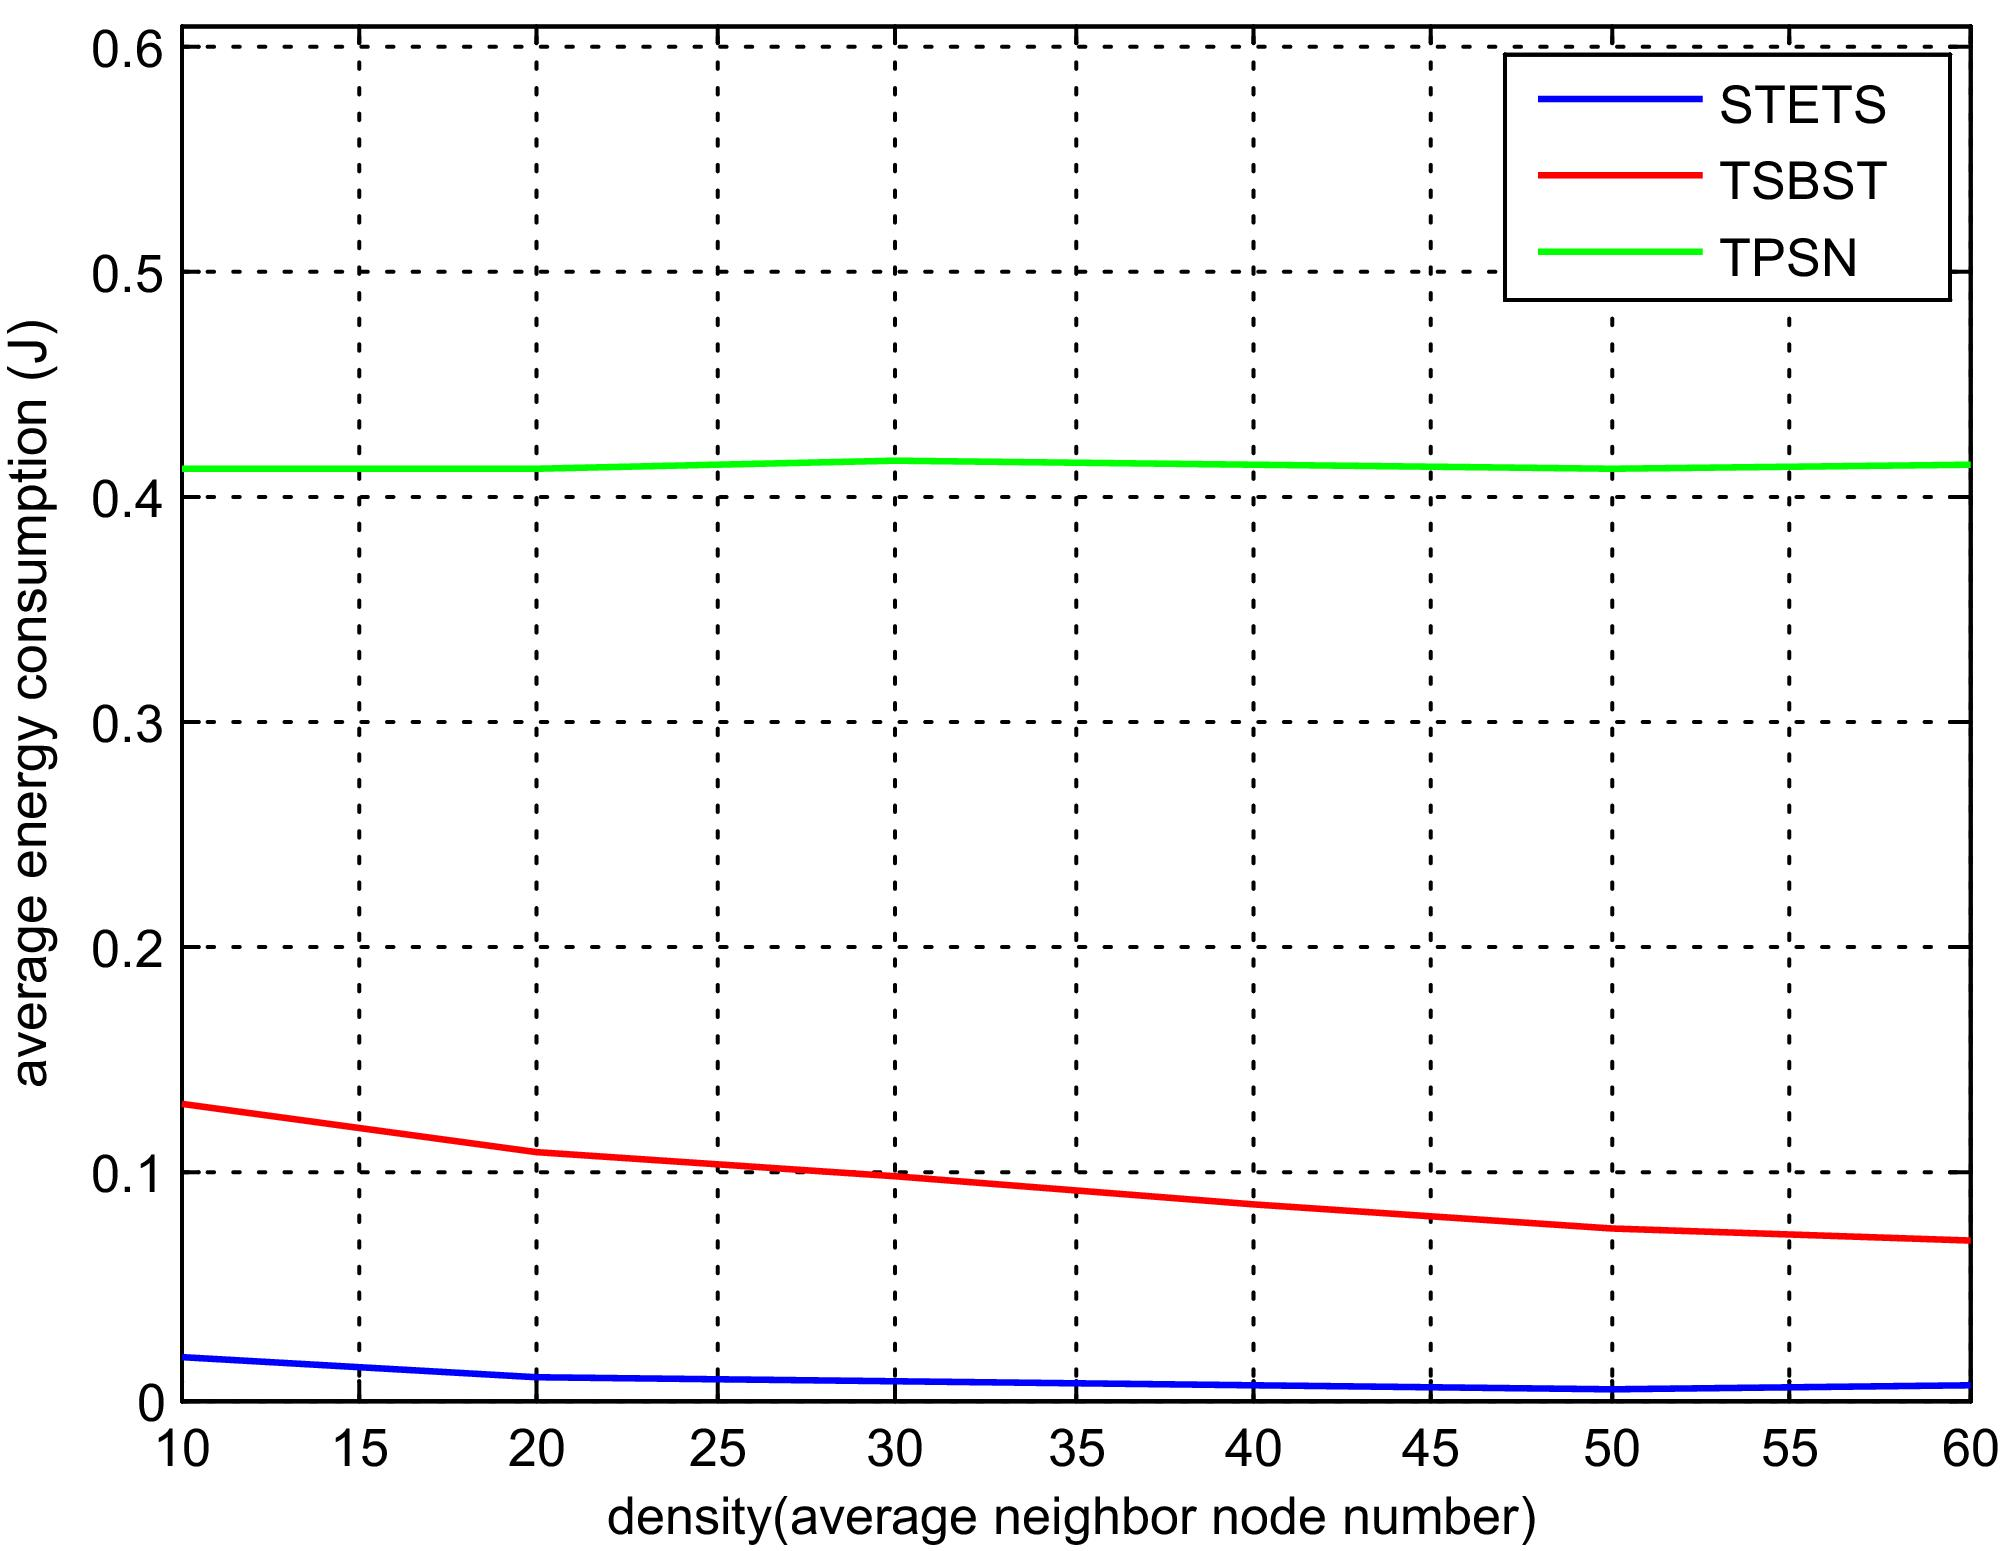
\includegraphics[width=2.5in]{fig3.jpg}
\caption{Average energy consumption}
\label{fig_sim}
\end{figure}


\subsection{Broadcast number and Energy Consumption}
Figure~3 shows the average energy consumption of each node. As we discussed in section 1, the major source of energy consumption in WSNs is the processes of sending and receiving messages. Thus, the more broadcasts are during the time synchronization, the more energy is consumed by each node.

The TPSN first creates a spanning tree of the network using flooding and then performs two-way message exchange along the edges. If there are N sensor nodes in the WSN, it takes 3N broadcasts during one single round of time synchronization. In contrast, the necessary broadcast number to perform TSBST during one single round of time synchronization is between N and 2N. The number would decline with the growth of network density. In STETS, the required broadcast number is always below N which indicates lower energy consumption than other two approaches. As the network density increases, the number of BNs will decrease. Therefore the broadcast number will further decline and energy consumption will also decrease. This means our approach is suitable for densely connected network.


\subsection{Local time synchronization error and global time synchronization error}
In our simulation, local time synchronization error is one-hop time synchronization error. Global time synchronization error is the time synchronization error between $b_{0}$ and other nodes in the WSN. It is very important to compare global time synchronization error since WSNs are usually multi-hop networks. We measure the local and global time synchronization error in WSNs at density 50.


\begin{figure}[t]
\centering
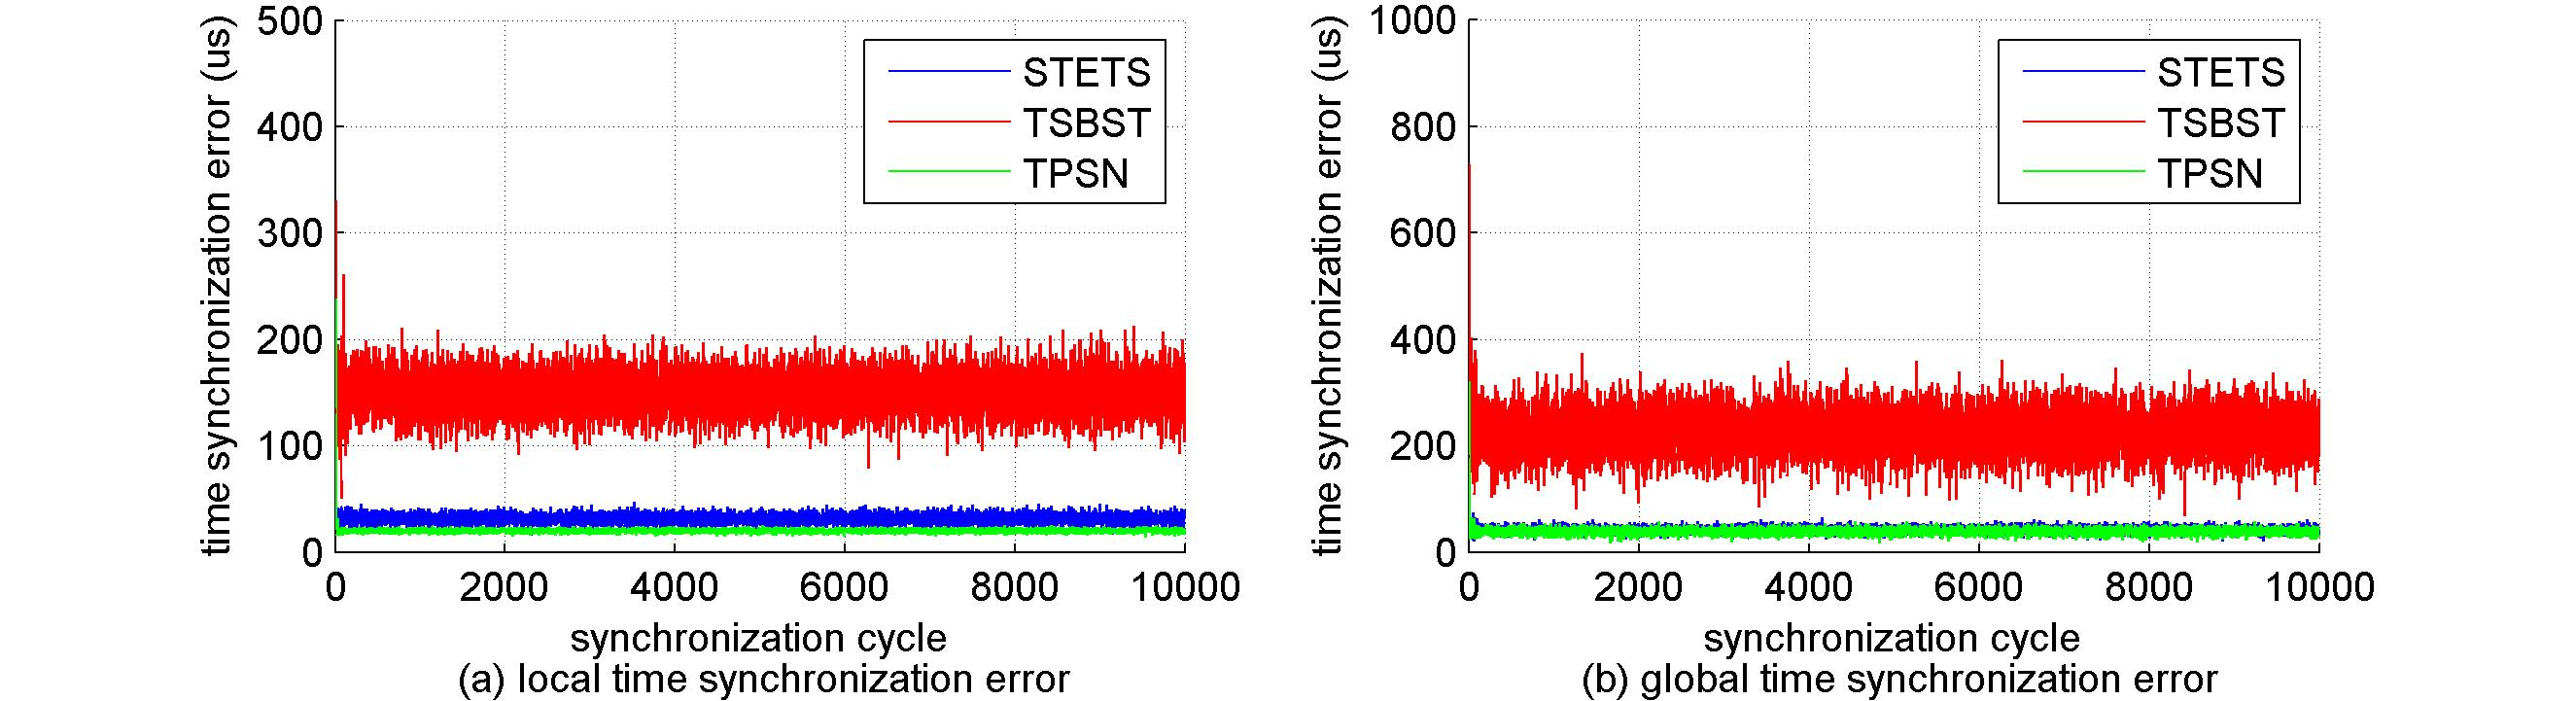
\includegraphics[width=\textwidth]{fig4.jpg}
\caption{Average BN and PN time synchronization error}
\label{fig_sim}
\end{figure}


Figure~4(a) is the comparison on local time synchronization error. Each point represents the average local time error of one single cycle of time synchronization. Figure~4(b) is the comparison on global time synchronization error. It can be seen from the two figures that both local and global time synchronization error of TSBST are much greater than those of STETS and TPSN. The time synchronization error of STETS and TPSN is similar. However, the energy consumption of TPSN is much higher than that of STETS, more than 10 times. This should be emphasized since energy-efficiency is an important issue for WSNs.


\section{Conclusion}
Most of the time synchronization approaches in WSNs suffer from high communication overheads when pursuing high accuracy. In this paper, we addressed this problem and proposed an approach, namely STETS based on spanning tree structure for WSNs. It combines two types of time synchronization, namely SRP and RRP in order to achieve energy-efficiency. We compare STETS with TPSN and TSBST by simulating them on NS-2. The results show that the energy consumption of our approach is much lower than other two approaches and the time synchronization error is similar to the TPSN. Moreover, our approach is effective especially in densely connected WSNs. A major disadvantage of STETS is that the time synchronization accuracy cannot surpass the accuracy of some existent approaches such as TPSN. We will still further our research on how to improve time synchronization accuracy in order to present a more accurate time synchronization approach with low energy consumption in the future.


\section{Acknowledgment}
This work was supported in part by Natural Science Foundation of P.R. China (Grant No. 61202443 and Grant
No. 61272524), and the Fundamental Research Funds for the Central Universities (No. DUT13JS07)..

\begin{thebibliography}{11}
\bibitem{1} M. Bhende, S. J. Wagh, A. Utpat. A quick survey on wireless sensor networks. 2014 4th International Conference on Communication Systems and Network Technologies, CSNT 2014, Bhopal, India, 7-9 Apr. 2014, pp. 160-167.
\bibitem{2} O. Gurcan, K. S. Yildirim. Self-organizing time synchronization of wireless sensor networks with adaptive Value Trackers. 2013 IEEE 7th International Conference on Self-Adaptive and Self-Organizing Systems, SASO 2013, Philadelphia, PA, United states, 9-13 Sept. 2013, pp. 91-100.
\bibitem{3} J. Elson, L. Girod, D. Estrin. Fine-grained network time synchronization using reference broadcasts. ACM SIGOPS Operating Systems Review, vol. 36, n. SI, pp. 147-163, 2002.
\bibitem{4} M. L. Sichitiu, C. Veerarittiphan. Simple, accurate time synchronization for wireless sensor networks. Wireless Communications and Networking, 2003. WCNC 2003. 2003 IEEE (Volume:2), New Orleans, LA, USA, 20-20 Mar. 2003, pp. 1266-1273.
\bibitem{5} S. Ganeriwal, R. Kumar, M. B. Srivastava. Timing-sync protocol for sensor networks. Proceedings of the 1st international conference on Embedded networked sensor systems. ACM, Los Angeles, California, 05 Nov. 2003, pp. 138-149.
\bibitem{6} L. M. He. Time synchronization based on spanning tree for wireless sensor networks. Wireless Communications, Networking and Mobile Computing, 2008. WiCOM'08. 4th International Conference on. IEEE, Dalian, 12-14 Oct. 2008, pp. 1-4.
\bibitem{7} I. Skog, P. H\"{a}ndel. Synchronization by two-way message exchanges: Cram\'{e}r-Rao bounds, approximate maximum likelihood, and offshore submarine positioning. IEEE Transactions on Signal Processing, vol. 58, n. 4, pp. 2351-2362, 2010.
\bibitem{8} W. Q. Hui, L. T. Ting, L. M. Long, W. L. Feng. Research on the WSN Node Localization Based on TOA. Journal of Applied Mathematics, vol. 2013, n. 706064, pp. 706064-706070, 2013.
\bibitem{9} P. Singh, S. Agrawal. TDOA Based Node Localization in WSN Using Neural Networks. 2013 International Conference on Communication Systems and Network Technologies (CSNT 2013), Gwalior, India, 6-8 Apr. 2013, pp. 400-404.
\bibitem{10} V. Daiya, J. Ebenezer, S.A.V.S. Murty, B. Experimental analysis of RSSI for distance and position estimation. 2011 International Conference on Recent Trends in Information Technology (ICRTIT 2011), Chennai, Tamil Nadu, India, 3-5 Jun. 2011, pp. 1093-1098.




%\bibitem{1} G. Fersi, W. Louati, M. B. Jemaa. Distributed Hash table-based routing and data management in wireless sensor networks: a survey. Wireless networks, vol. 19, n. 2, pp. 219-236, 2013.
%\bibitem{2} A. Aziz, Y. Sekercioglu, P. Fitzpatrick, M. Ivanovich. A survey on distributed topology control techniques for extending the lifetime of battery powered wireless sensor networks. Communications Surveys {\&} Tutorials, IEEE, vol. 15, n. 1, pp. 121-144, 2013.
%\bibitem{3} M. A. Razzaque, C. Bleakley, S. Dobson. Compression in wireless sensor networks: A survey and comparative evaluation. ACM Transactions on Sensor Networks (TOSN), vol. 10, n. 1, pp. 1-44, 2013.
%\bibitem{4} D. Butler. 2020 computing: Everything, everywhere. Nature, vol. 440, n. 7083, pp. 402-405, 2006.
%\bibitem{5} D. Estrin. Embedded everywhere: A research agenda for networked systems of embedded computers. Washington, D.C.: National Academy Press, 2001.
%\bibitem{6} M. P. Durisic, Z. Tafa, G. Dimic, V. Milutinovic. A survey of military applications of wireless sensor networks. Embedded Computing (MECO), 2012 Mediterranean Conference on. IEEE, Bar, 19-21 Jun. 2012, pp. 196-199.
%\bibitem{7} D. Kim, H. Park, S. Yoo. Performance evaluation of routing protocols for wireless sensor networks in military scenarios. Ubiquitous and Future Networks (ICUFN), 2011 Third International Conference on. IEEE, Dalian, 15-17 Jun. 2011, pp. 101-106.
%\bibitem{8} C. J. Rankine, A. Sanchez-Azofeifa, M. M. do Esp\'{\i}rito-Santo, M.T.S. Viera. Optical wireless sensor networks observe leaf phenology and photosynthetic radiation interception in a Brazilian tropical dry forest. Geoscience and Remote Sensing Symposium (IGARSS), 2012 IEEE International. IEEE, Munich, 22-27 Jul. 2012, pp. 6914-6915.
%\bibitem{9} K. Smarsly. Agricultural ecosystem monitoring based on autonomous sensor systems. Agro-Geoinformatics (Agro-Geoinformatics), 2013 Second International Conference on. IEEE, Fairfax, VA, 12-16 Aug. 2013, pp. 402-407.
%\bibitem{10} L. Dong, L. Wei, H. Chunli, H. Changcheng, C. Li. Wireless sensor networks in relic protection: Deployment methodology and cross-layer design. High Technology Letters, vol. 15, n. 11, pp. 59-64, 2009.
%\bibitem{11} H. Mart\'{\i}n, A. M. Bernardos, L. Bergesio, P. Tarrio. Analysis of key aspects to manage wireless sensor networks in ambient assisted living environments. Applied Sciences in Biomedical and Communication Technologies, 2009. ISABEL 2009. 2nd International Symposium on. IEEE, Bratislava, 24-27 Nov. 2009, pp. 1-8.
%\bibitem{12} W. Suntiamorntut, S. Charoenpanyasak, J. Ruksachum. An elderly assisted living system with wireless sensor networks. Wireless and Mobile Networking Conference (WMNC), 2011 4th Joint IFIP. IEEE, Toulouse, 26-28 Oct. 2011, pp. 1-6.
%\bibitem{13} K. Park, E. Becker, J. K. Vinjumur, Z. Le, F. Makedon. Human behavioral detection and data cleaning in assisted living environment using wireless sensor networks. Proceedings of the 2nd International Conference on PErvasive Technologies Related to Assistive Environments. ACM, Corfu, Greece, 09 Jun. 2009, pp. 1-8.
%\bibitem{14} J. Heidemann, W. Ye, J. Wills, A. Syed, Y. Li. Research challenges and applications for underwater sensor networking. Wireless Communications and Networking Conference, 2006. WCNC 2006. IEEE (Volume:1). Las Vegas, NV, 3-6 April 2006, pp. 228-235.
%\bibitem{15} B. Sundararaman, U. Buy, A. D. Kshemkalyani. Clock synchronization for wireless sensor networks: a survey. Ad Hoc Networks, vol. 3, n. 3, pp. 281-323, 2005.
%\bibitem{16} M. L. Sichitiu, C. Veerarittiphan. Simple, accurate time synchronization for wireless sensor networks. Wireless Communications and Networking, 2003. WCNC 2003. 2003 IEEE (Volume:2), New Orleans, LA, USA, 20-20 Mar. 2003, pp. 1266-1273.
%\bibitem{17} J. Elson, L. Girod, D. Estrin. Fine-grained network time synchronization using reference broadcasts. ACM SIGOPS Operating Systems Review, vol. 36, n. SI, pp. 147-163, 2002.
%\bibitem{18} S. Ganeriwal, R. Kumar, M. B. Srivastava. Timing-sync protocol for sensor networks. Proceedings of the 1st international conference on Embedded networked sensor systems. ACM, Los Angeles, California, 05 Nov. 2003, pp. 138-149.
%\bibitem{19} L. M. He. Time synchronization based on spanning tree for wireless sensor networks. Wireless Communications, Networking and Mobile Computing, 2008. WiCOM'08. 4th International Conference on. IEEE, Dalian, 12-14 Oct. 2008, pp. 1-4.
%\bibitem{20} I. Skog, P. H\"{a}ndel. Synchronization by two-way message exchanges: Cram\'{e}r-Rao bounds, approximate maximum likelihood, and offshore submarine positioning. IEEE Transactions on Signal Processing, vol. 58, n. 4, pp. 2351-2362, 2010.
%\bibitem{21} G. Cena, S. Scanzio, A. Valenzano, C. Zunino. The reference-broadcast infrastructure synchronization protocol. 2012 IEEE 17th International Conference on Emerging Technologies and Factory Automation, ETFA 2012, Krakow, Poland, 17-21 Sept. 2012, pp. 1-5.
%\bibitem{22} S. Jain, Y. Sharma. Optimal Performance Reference Broadcast Synchronization~(OPRBS) for time~synchronization~in wireless sensor networks. 2011 International Conference on Computer, Communication and Electrical Technology, ICCCET 2011, Maruthakulam, India, 18-19 Mar. 2011, pp. 171-175.
%\bibitem{23} J. Elson, D. Estrin. Time synchronization for wireless sensor networks. In Proceedings of the 15th International Parallel and Distributed Processing Symposium (IPDPS-01). IEEE Computer Society, 23-27 Apr. 2001, pp. 1-6.
%\bibitem{24} Z. Zhong, P. Chen, T. He. On-demand time synchronization with predictable accuracy. INFOCOM, 2011 Proceedings IEEE, Shanghai, 10-15 Apr. 2011, pp. 2480-2488.
%\bibitem{25} S. Y. Kasim, K. Aylin. External Gradient Time Synchronization in Wireless Sensor Networks. IEEE Transactions on Parallel and Distributed System, vol. 25, n. 3, pp. 1-9, 2014.
%\bibitem{26} W. Q. Hui, L. T. Ting, L. M. Long, W. L. Feng. Research on the WSN Node Localization Based on TOA. Journal of Applied Mathematics, vol. 2013, n. 706064, pp. 706064-706070, 2013.
%\bibitem{27} P. Singh, S. Agrawal. TDOA Based Node Localization in WSN Using Neural Networks. 2013 International Conference on Communication Systems and Network Technologies (CSNT 2013), Gwalior, India, 6-8 Apr. 2013, pp. 400-404.
%\bibitem{28} V. Daiya, J. Ebenezer, S.A.V.S. Murty, B. Experimental analysis of RSSI for distance and position estimation. 2011 International Conference on Recent Trends in Information Technology (ICRTIT 2011), Chennai, Tamil Nadu, India, 3-5 Jun. 2011, pp. 1093-1098.
%\bibitem{29} P. Jacquet, A. Meraihi Naimi, G. Rodolakis. Asymptotic delay analysis for cross-layer delay-based routing in ad hoc networks. Advances in Multimedia, vol. 2007, n. 90879, pp. 1-11, 2007.

\end{thebibliography}
%\begin{verbatim}
%\begin{thebibliography}{}  % (do not forget {})
%.
%.
%\bibitem[1982]{clar:eke}
%Clarke, F., Ekeland, I.:
%Nonlinear oscillations and boundary-value problems for
%Hamiltonian systems.
%Arch. Rat. Mech. Anal. {\bfseries 78} (1982) 315--333
%.
%.
%\end{thebibliography}
%\end{verbatim}
%{\itshape Sample Output}
%\bibauthoryear
%
\end{document}
